\documentclass{article}
\usepackage{graphicx}
\usepackage{url,parskip} 	%other packages for formatting
\usepackage[usenames,dvipsnames]{xcolor}
\usepackage{supertabular} 				%for Grades
\usepackage{titlesec}					%custom \section

%Setup hyperref package, and colours for links
\usepackage{hyperref}
\definecolor{linkcolour}{rgb}{0,0.2,0.6}
\hypersetup{colorlinks,breaklinks,urlcolor=linkcolour, linkcolor=linkcolour}

\titleformat{\section}{\Large\scshape\raggedright}{}{0em}{}[\titlerule]
\titlespacing{\section}{0pt}{3pt}{3pt}

\def\LOGO{%
\begin{picture}(0,0)\unitlength=1cm
\put (0,-4) {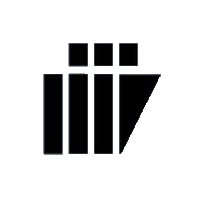
\includegraphics[scale=0.8]{logo_iiitv.png}}
\end{picture}
}
\usepackage{geometry}
\geometry{top=15mm,bottom=15mm,left=15mm,right=15mm}

\begin{document}
\begin{minipage}{\linewidth}
\LOGO\\
\end{minipage}
\begin{flushright}
\begin{minipage}{13cm}
%------------------------------------------Personal Data---------------------------------------------%
\begin{huge}\textbf{Shubham Subhankar Sharma }\\  \end{huge}
\begin{large}
\textbf{Indian Institute of Information Technology, Vadodara\\ \\}
\textbf{Email:}shubhamshubhankar.sharma@gmail.com \hspace*{5mm}\textbf{DOB}: 29/05/1994\\
\textbf{Address}:Hno.19,Veer Sawarkar Nagar,Phase1,Bareilly,UP,India(243005)
\end{large}
\end{minipage}
\end{flushright}

%Section: Education
\section{Education}
\begin{tabular}{lllc}
\textbf{Degree}&\textbf{Institute}&\textbf{Year}&\textbf{CPI/Aggregate}\\
B.Tech.& Indian Institute of Information Technology, Vadodara, India & 2013-2017 &  8.43\\
Intermidiate/+2 & Kendriya Vidyalaya N.E.R Bareilly, U.P, India & 2011-2014 & 91.8\%\\
High School & Kendriya Vidyalaya Lokra, Sonitpur, Assam, India & 2009-2010 & 9.8 \\
\end{tabular}

%Section: Skills
\section{Skills}
\begin{tabular}{ll}
\textbf{Expertise Area:} C++, Java, PostgreSQL, OOPs, Algorithm Design and Analysis, Canny Edge Detection \\ \\
\textbf{Area(s) of Interest:} Information Retrieval, Big data(Hadoop and MapReduce Architecture), Internet Security,\\ NLP, SQL injection and Brute Force Attack, Digital Image Processing \\ \\
\textbf{Programming Language(s):} C++, C, Java, Matlab, OpenCV\\ \\
\textbf{Tools and Technologies/SDK(s):} Wireshark, Tshark, Joomla, Latex, word2vec(NLP)  \\ \\
\textbf{Database:} PostgreSQL, MySQL, Database Design and Analysis\\ \\
\textbf{Electives:} Graph Theory and Optimization, Science Technology and Society, Science Fiction, Economics\\ \\
\end{tabular}


%Section: Projects
\section{Projects}
\begin{large}\textbf{Hadoop, MapReduce paradigm and its Applications }\end{large}\\
\textbf{Indian Institute of Information Technology, Vadodara}\\
\textbf{Instructor: Dr. Prasenjit Mazumder, Professor, DAIICT Gandhinagar, India}\hfill{} \textbf{Team size 2} \\
In this project, we installed  Hadoop( an open-source framework that allows to store and process big data in a distributed environment across clusters of computers using simple programming models) on a cluster of three computers. One as master and two acting as a slave. We implemented Least common subsequence problem for generating summaries and DNA matching in hadoop.  \\
\textbf{My contribution}: Installation of the system and designing and implementing algorithm for LCS in java.\\


\begin{large}\textbf{Brute Force and SQL Injection Attack detection and prevention using Wireshark }\end{large} \\
\textbf{Indian Institute of Information Technology, Vadodara}\\
\textbf{ Instructor : Dr. Jignesh Bhatt, professor, IIIT Vadodara, India } \hfill{}
\textbf{Team size 3} \\
In this project, we developed a module for doing Brute Force Attack (for getting username and password) and did SQL Injection Attack on a isolated system using a single system as victim and multiple system as 	In this project, we made a UG Convener Website using the Joomla
CMS(Content Management System). This site acts as a communication medium between the Dean of the institute and all the other students, Alumni, Staff and the Faculty. Anyone can directly contact and interact with Dean after registration. And dean can give notifications and further information about his actions. \\
\textbf{My contribution}: Designer and Content Writer of the website.\\

%\begin{large}\textbf{Implementing Newton Rhapson Method for solving Real and Complex Equation }\end{large} \\
%\textbf{Indian Institute of Information Technology, Vadodara}\\
%\textbf{Instructor : Dr. Pratik Shah,Associate Professor, Indian Institute of Information Technology, Vadodara, India}\hfill{}
%\textbf{Team size 5}\\
%In this project,we implemented Newton Rhapson Method for solving Real and Complex Equation. Using octave and C languages, we plotted the positions of the imaginary and real roots on the graphs producing fractal images.


\begin{large}\textbf{College Management System }\end{large} \\
\textbf{Indian Institute of Information Technology, Vadodara}\\
\textbf{Instructor : Dr. Asim Banerjee, Professor, DAIICT Gandhinagar, India}\hfill{}
\textbf{Team size 9} \\
CMS is a standalone Intranet based application that aims at providing information to all the levels of management within an organization.It mainly focuses on administration, academics, hostel and mess related issues. It is made using the MVC model. I was responsible for requirement gathering, backend programming using PHP and documentation of SRS, User Manual and Integration Testing in this project.\\
\textbf{My contribution}: Backend developing and Requirement gathering in the college.\\


\begin{large}\textbf{Canny Edge Detection and Harris Corner Detection }\end{large} \\
\textbf{Indian Institute of Information Technology, Vadodara}\\
\textbf{Instructor : Dr. Jignesh Bhatt, Professor, IIIT Vadodara, India}\hfill{} 
In this project, I implemented Canny Edge Detection and Harris Corner Detection for feature extraction in Matlab. The purpose of line detection algorithm is to compress the image while preserving the structural properties of the image. I am going to use these techniques in my further works for OCR(Optical Character Recognition) for Handwritten and Printed text.\\

%\begin{large}\textbf{ensureIntern }\end{large} \\
%\textbf{Indian Institute of Information Technology, Vadodara}\\
%\textbf{ Instructor : Dr. Pokhar Mal Jat, professor, DAIICT, Gandhinagar, India }\\
%\textbf{Team size 3} \\
%We built ensureIntern as our web technology project. This website provides student all the %information about the internship. Starting from where to apply for the internship on the basis %of the students skill set and interest, what should be the format of resume, how to prepare %for the interview and the guidelines for the behaivior during the internship. This website is %made in MVC(Model View Controller) model using servlet and JSP.

%Section: Internships
\section{Training}
\begin{large}\textbf{MIT Media Lab Workshop(Innovative Design) in Synchronous Tools Track}\\ \\
\end{large}
\textbf{Pandit Deendayal Petroleum Universiy}\\
\textbf{Mentor: Tomer Weller and Jonathan Bobrow}
In this workshop, I explored various technology like tessel(microcontroller), google glass, 3d printer, oculas etc. I learnt about how to do paper prototyping, pitch your product and make it presentable. I also learned how to collaborate with enthusiasts from different field and work as a team.\\

\begin{large}\textbf{Cloud Computing Workshop at Robotryst}\\ \\
\end{large}
\textbf{IIT Delhi} \\
\textbf{Mentor: Madhur Malhotra}\\
In this workshop, I learnt about the ins and outs of cloud computing starting from virtualisation to handling and working with IaaS, PaaS, SaaS like Amazon EC2, Google AppEngine.\\




%Section: Position(s) of Responsibility
\section{Position(s) of Responsibility}
\begin{itemize}
\item School Captain, Kendriya Vidyalaya NER Bareilly (15 September 2011 - 20 April 2012)
\item Sports Committee Head, IIIT Vadodara (20 August 2013 - 30 September 2014)
\item Teaching Assistant(TA) for DBMS course, IIIT Vadodara for the second year students.(2 February 2016 - till date)
\end{itemize}

%Section: Interests and Activities
\section{Interests and Activities}
\begin{itemize}
\item Sports attract me. It fills me with energy. I love to play football, table tennis, badminton, cricket and  volleyball. I have represented my state for two years in table tennis at the nationals.
\item Singing songs and listening to them helps me to relax and fills me with energy.
\item I love to travel and discover new and adventurous tourist destination. 
\item I am a foody guy. Love to try new dishes and recipes.
\item Sketching cartoons and sceneries. 
\end{itemize}



\vspace*{1cm}
\textbf{Declaration} : I hereby declare that all the details furnished above are true to the best of my knowledge and belief.
\end{document}
